\chapter{Specifikacija programske potpore}
		
	\section{Funkcionalni zahtjevi}


			
			\noindent \textbf{Dionici:}
			
			\begin{packed_enum}
				
				\item Primarni dionici:
				
				\begin{packed_enum}
					\item Naručitelj
					\item Razvojni tim
					\item Rukovoditelji razvoja
					\item Strateški klijenti
					\item Super administrator
					\item Administrator
				\end{packed_enum}
				
				\item Sekundarni dionici:	
				
				\begin{packed_enum}
					\item Sudionici konferencije
					\item Zaposlenici konferencije
					\item Autori	
				\end{packed_enum}		
				
			\end{packed_enum}
			
			\noindent \textbf{Akteri i njihovi funkcionalni zahtjevi:}
			
			
			\begin{packed_enum}
				\item Neregistrirani posjetitelji konferencije
				
			\begin{quote}
				Neregistrirani posjetitelji konferencije imaju mogućnost pregledavanja stručnih postera svih prijavljenih sudionika pomoću lozinke dobivene na konferenciji i dodatna registracija u sustav po želji.
			\end{quote}
				
				\item Registrirani posjetitelji konferencije
				
		\begin{quote}
			Registrirani posjetitelji konferencije imaju dodatnu mogućnost glasanja za najbolji stručni poster uključujući pristup rezultatima glasovanja kako bi vidjeli koji poster osvaja najviše glasova kao i uživo praćenje trenutnih događanja u glavnoj konferencijskoj dvorani. Također imaju priliku vidjeti promotivne materijale pokrovitelja konferencije te podatke o trenutnim vremenskim uvjetima i vremenskoj prognozi za navedenu lokaciju. Po završetku, registrirani posjetitelji konferencije će moći pregledavati i preuzimati objavljene fotografije konferencije.
		\end{quote}
		
				\item Super administrator
				\begin{quote}
					Super Administrator ima mogućnost davanja administrator uloga već postojećim računima.
				\end{quote}
				
				\item Administrator
				\begin{quote}
					Administrator ima mogućnost kreiranja nove konferencije. Prilikom kreiranja konferencije, administrator može odabrati njezin naziv, opis konferencije, mjesto održavanja, njezin početak kao i njezin kraj. Inicijalnu lozinku konferencije sustav automatski generira.
				\end{quote}
				
				\item Autori
				\begin{quote}
					Autori su glavni sudionici konferencije koji će nastupati. Oni prije početka konferencije elektroničkom poštom dostavljaju sve potrebne materijale (postere) sistemskom administratoru. Također, nakon završetak konferencije elektroničkom poštom dobivaju informaciju o njihovom rangu kao i pozivnicu za dodjelu nagrada.
				\end{quote}
				
				\item Pokrovitelji
				\begin{quote}
					Pokrovitelji konferenciju financiraju samu konferenciju i dostavljaju promotivne materijale sistemskom administratoru koji će se prikazivati registriranim posjetiteljima
				\end{quote}
				
				
				\item \textit{Aplikacija i baza podataka}
				\begin{quote}
					\textit{Pasivni faktori same funkcionalnosti aplikacije kao i spremanja podataka}
				\end{quote}
			\end{packed_enum}
			
			\eject 
			
			
				
			\subsection{Obrasci uporabe}
				
				\textbf{\textit{dio 1. revizije}}
				
				\subsubsection{Opis obrazaca uporabe}
					\textit{Funkcionalne zahtjeve razraditi u obliku obrazaca uporabe. Svaki obrazac je potrebno razraditi prema donjem predlošku. Ukoliko u nekom koraku može doći do odstupanja, potrebno je to odstupanje opisati i po mogućnosti ponuditi rješenje kojim bi se tijek obrasca vratio na osnovni tijek.}\\
									
					
					\noindent \underbar{\textbf{UC1 - Prijava u sustav odgovarajućom lozinkom}}
					\begin{packed_item}
						
						\item \textbf{Glavni sudionik: } Svi posjetitelji konferencije
						\item  \textbf{Cilj:} Prijava u sustav
						\item  \textbf{Sudionici:} Aplikacija i baza podataka
						\item  \textbf{Preduvjet:} Odgovarajuća lozinka dostupna svim posjetiteljima konferencije
						\item  \textbf{Opis osnovnog tijeka:}
						
						\item[] \begin{packed_enum}
							
							\item Posjetitelj upisuje lozinku dobivenu na konferenciji 
							\item Sustav provjerava odgovara li kriptografski sažetak lozinke upisane od strane korisnika sa onom u bazi podataka
							\item Ukoliko je lozinka točna, posjetitelj se uspješno prijavljuje u aplikaciju
							\item Prijavljenom korisniku se otvara nova stranica
						\end{packed_enum}
						
						\item  \textbf{Opis mogućih odstupanja:}
						
						\item[] \begin{packed_item}
							
							\item[1.a] Posjetitelj je upisao pogrešnu lozinku
							\item[] \begin{packed_enum}
								
								\item Posjetitelj dobiva obavijest od strane aplikacije kako je njegova lozinka neispravna
								\item Od posjetitelja se traži da opet upiše točnu lozinku
								
							\end{packed_enum}
						
							
						\end{packed_item}
					\end{packed_item}
					
					\noindent \underbar{\textbf{UC2 - Odjava prijavljenog korisnika}}
					\begin{packed_item}
						
						\item \textbf{Glavni sudionik: }Korisnik
						\item  \textbf{Cilj:} Odjava prijavljenog korisnika
						\item  \textbf{Sudionici:} Aplikacija i baza podataka
						\item  \textbf{Preduvjet:} Korisnik je prijavljen u sustav
						\item  \textbf{Opis osnovnog tijeka:}
						
						\item[] \begin{packed_enum}
							
							\item Posjetitelj se uspješno prijavio u sustav odgovarajućom lozinkom
							\item Korisnik je pritisnuo gumb za odjavu prijavljenih korisnika iz sustava 
							\item Sustav ga uspješno odjavljuje i vraća na početnu stranicu
							
						\end{packed_enum}
						
						\item  \textbf{Opis mogućih odstupanja:}
						
						\item[] \begin{packed_item}
							
							\item[1.a] Korisnik se nije uspješno prijavio u sustav
							\item[] \begin{packed_enum}
								
								\item Od strane korisnika se zahtjeva da se prijavi u sustav odgovarajućom lozinkom
								
							\end{packed_enum}
							
							
						\end{packed_item}
					\end{packed_item}
					
					
					\noindent \underbar{\textbf{UC3 - Pregledavanje stručnih postera prijavljenih korisnika}}
					\begin{packed_item}
						
						\item \textbf{Glavni sudionik: }Korisnik
						\item  \textbf{Cilj:} Pregledavanje stručnih postera
						\item  \textbf{Sudionici:} Aplikacija i baza podataka
						\item  \textbf{Preduvjet:} Korisnik je prijavljen u sustav
						\item  \textbf{Opis osnovnog tijeka:}
						
						\item[] \begin{packed_enum}
							
							\item Aplikacija dohvaća potrebne materijale i postere iz baze podataka
							\item Korisnik ima mogućnost pregledavanja stručnih postera
							
						\end{packed_enum}
						
					\end{packed_item}
					
				
				
				
				\noindent \underbar{\textbf{UC4 - Registracija u sustav prijavljenih korisnika}}
				\begin{packed_item}
					
					\item \textbf{Glavni sudionik: }Korisnik
					\item  \textbf{Cilj:} Registracija u sustav već prijavljenih korisnika
					\item  \textbf{Sudionici:} Aplikacija i baza podataka
					\item  \textbf{Preduvjet:} Korisnik je prijavljen u sustav
					\item  \textbf{Opis osnovnog tijeka:}
					
					\item[] \begin{packed_enum}
						
						\item Korisnik je pritisnuo gumb za registraciju u sustav
						\item Korisniku se otvara nova stranica sa poljem za upis elektroničke pošte i nove lozinke
						\item Sustav provjerava valjanost upisane elektroničke pošte kao i lozinke
						\item Elektronička pošta registriranog korisnika se sprema u bazu podataka dok se upisana lozinka kriptira te se njezin sažetak sprema u bazu 

					\end{packed_enum}
					
					\item  \textbf{Opis mogućih odstupanja:}
					
					\item[] \begin{packed_item}
						
						\item[3.a] Pogrešan unos elektroničke pošte
						\item[] \begin{packed_enum}
							
							\item Sustav provjerava ispravnost unesene elektroničke pošte te ukoliko je kriva, obavještava korisnika o ispravnom napisanom obliku
							\item Korisnik upisuje ispravnu elektroničku poštu
							
						\end{packed_enum}
						\item[3.b] Pogrešan unos lozinke
						\item[] \begin{packed_enum}
							
							\item Sustav provjerava ispravnost unesene lozinke te ukoliko je kriva, obavještava korisnika o ispravnom napisanom obliku
							\item Korisnik upisuje ispravnu lozinku
							
						\end{packed_enum}
						
						\item[4.a] Korisnik je već prijavljen u sustav
						\item[] \begin{packed_enum}
							
							\item Sustav provjerava postoji li već registriran korisnik iste elektroničke pošte
							\item Sustav odbija registraciju korisnika te ga obavještava kako je korisnik već registriran 
							
						\end{packed_enum}
						
					\end{packed_item}
				\end{packed_item}
				
				
				
				\noindent \underbar{\textbf{UC5 - Odjava registriranog korisnika}}
				\begin{packed_item}
					
					\item \textbf{Glavni sudionik: }Korisnik
					\item  \textbf{Cilj:} Odjava iz sustava registriranog korisnika
					\item  \textbf{Sudionici:} Aplikacija i baza podataka
					\item  \textbf{Preduvjet:} Registrirani korisnik je prijavljen u sustav
					\item  \textbf{Opis osnovnog tijeka:}
					
					\item[] \begin{packed_enum}
						
						\item Korisnik je pritisnuo gumb za odjavu registriranih korisnika iz sustava 
						\item Sustav ga uspješno odjavljuje i vraća na početnu stranicu prijavljenih korisnika
						
					\end{packed_enum}
					
				\end{packed_item}
				
				
				\noindent \underbar{\textbf{UC6 - Glasanje za najbolji stručni poster konferencije}}
				\begin{packed_item}
					
					\item \textbf{Glavni sudionik: }Korisnik
					\item  \textbf{Cilj:} Glasanje za najbolji stručni poster konferencije
					\item  \textbf{Sudionici:} Aplikacija i baza podataka
					\item  \textbf{Preduvjet:} Glasovanje je moguće samo registriranim korisnicima tijekom određenog vremenskog razdoblja koje je određeno danima i vremenom održavanja konferencije
					\item  \textbf{Opis osnovnog tijeka:}
					
					\item[] \begin{packed_enum}
						
						\item Registrirani korisnik pregledava objavljene stručne postere
						\item Nakon što registrirani korisnik odabere njemu najbolji poster, ima mogućnost glasanja za taj poster
						\item Registrirani korisnik pritišće gumb za glasanje određenog postera
						\item Aplikacija sprema u bazu podataka taj glas i označava da je taj korisnik glasao i da više nema mogućnost glasanja

					\end{packed_enum}
					
					\item  \textbf{Opis mogućih odstupanja:}
					
					\item[] \begin{packed_item}
						
						\item[3.a] Registrirani korisnik pritišće gumb za glasanje određenog postera van vremenskom razdoblja predviđenog za glasanje
						\item[] \begin{packed_enum}
							
							\item Registrirani korisnik pritišće gumb za glasanje određenog poster
							\item Sustav ga obavještava kako ne može glasati budući da glasovanje još nije započeto te mu javlja točno vrijeme početka glasanja
							
						\end{packed_enum}
						
						\item[3.b] Registrirani korisnik pritišće gumb za glasanje drugog postera
						\item[] \begin{packed_enum}
							
							\item Registrirani korisnik pritišće gumb za glasanje određenog postera nakon što je već jednom glasao za neki drugi poster
							\item Sustav ga obavještava kako ne može glasati budući da već jednom glasao
							
						\end{packed_enum}
						
						
					\end{packed_item}
				\end{packed_item}
				
				
				\noindent \underbar{\textbf{UC7 - Povlačenje korisnikovog glasa stručnog postera}}
				\begin{packed_item}
					
					\item \textbf{Glavni sudionik: }Korisnik
					\item  \textbf{Cilj:} Povlačenje korisnikovog glasa stručnog postera
					\item  \textbf{Sudionici:} Aplikacija i baza podataka
					\item  \textbf{Preduvjet:} Povlačenje glasa je moguće samo registriranim korisnicima koji su već glasali tijekom određenog vremenskog razdoblja koje je određeno danima i vremenom održavanja konferencije
					\item  \textbf{Opis osnovnog tijeka:}
					
					\item[] \begin{packed_enum}
						
						\item Korisnik je odlučio promijeniti svoje mišljenje te želi povući svoj glas za već odabrani stručni poster
						\item Registrirani korisnik pritišće gumb za povlačenje glasa određenog postera
						\item Aplikacija briše iz baze podataka taj glas i označava taj korisnik može ponovno glasati
					\end{packed_enum}
					
					
				\end{packed_item}
				
				
				\noindent \underbar{\textbf{UC8 - Gledanje uživo prijenosa konferencije}}
				\begin{packed_item}
					
					\item \textbf{Glavni sudionik: }Korisnik
					\item  \textbf{Cilj:} Gledanje uživo prijenosa konferencije
					\item  \textbf{Sudionici:} Aplikacija i baza podataka
					\item  \textbf{Preduvjet:} Gledanje uživo prijenosa konferencije je moguće samo registriranim korisnicima tijekom određenog vremenskog razdoblja koje je određeno danima i vremenom održavanja konferencije
					\item  \textbf{Opis osnovnog tijeka:}
					
					\item[] \begin{packed_enum}
						
						\item Registrirani korisnik pritišće gumb za praćenje uživo prijenosa konferencije 
						\item Aplikacija dohvaća iz baze podataka potreban video prijenos te se korisniku prikazuje video prozor
					\end{packed_enum}
					
					\item  \textbf{Opis mogućih odstupanja:}
					
					\item[] \begin{packed_item}
						
						\item[1.a] Registrirani korisnik pritišće gumb za praćenje uživo prijenosa konferencije van vremenskom razdoblja predviđenog za uživo prijenos konferencije
						\item[] \begin{packed_enum}
							
							\item Registrirani korisnik pritišće gumb za praćenje uživo prijenosa konferencije 
							\item Sustav ga obavještava kako ne može gledati uživo prijenos konferencije budući da ono još nije započeto te mu javlja točno vrijeme početka konferencije
							
						\end{packed_enum}
				
						
					\end{packed_item}
				\end{packed_item}
				
				
				
				\noindent \underbar{\textbf{UC9 - Zatvaranje uživo prijenosa konferencije}}
				\begin{packed_item}
					
					\item \textbf{Glavni sudionik: }Korisnik
					\item  \textbf{Cilj:} Zatvaranje uživo prijenosa konferencije
					\item  \textbf{Sudionici:} Aplikacija i baza podataka
					\item  \textbf{Preduvjet:} Zatvaranje uživo prijenosa konferencije je moguće samo registriranim korisnicima koji gledaju uživo prijenos konferencije tijekom određenog vremenskog razdoblja koje je određeno danima i vremenom održavanja konferencije
					\item  \textbf{Opis osnovnog tijeka:}
					
					\item[] \begin{packed_enum}
						
						\item Registrirani korisnik pritišće gumb za Zatvaranje uživo prijenosa konferencije 
						\item Aplikacija zatvara video prozor
						
						
					\end{packed_enum}
					
				\end{packed_item}
				
				
				\noindent \underbar{\textbf{UC10 - Pregled poretka stručnih postera}}
				\begin{packed_item}
					
					\item \textbf{Glavni sudionik: }Korisnik
					\item  \textbf{Cilj:} Pregled poretka stručnih postera
					\item  \textbf{Sudionici:} Aplikacija i baza podataka
					\item  \textbf{Preduvjet:} Pregled poretka stručnih postera je dostupan svim registriranim korisnica po završetku konferencije i njenog glasanja
					\item  \textbf{Opis osnovnog tijeka:}
					
					\item[] \begin{packed_enum}
						
						\item Konferencija kao i njeno glasanje je završeno
						\item Aplikacija iz baze podataka dohvaća glasove stručnih postera te pokazuje poredak najboljih stručnih postera svim registriranim korisnima 
					\end{packed_enum}
					
					\item  \textbf{Opis mogućih odstupanja:}
					
					\item[] \begin{packed_item}
						
						\item[2.a] Poredak nije dostupan
						\item[] \begin{packed_enum}
							
							\item Prostor za poredak stručnih postera je prazan
							\item Glasanje kao i sama konferencija nisu još završeni te sustav obavještava korisnika o vremenu objave poretka
							
						\end{packed_enum}
				
						
					\end{packed_item}
				\end{packed_item}
				
				
				
				\noindent \underbar{\textbf{UC11 - Gledanje promotivnih materijala pokrovitelja}}
				\begin{packed_item}
					
					\item \textbf{Glavni sudionik: }Korisnik
					\item  \textbf{Cilj:} Gledanje promotivnih materijala pokrovitelja
					\item  \textbf{Sudionici:} Aplikacija i baza podataka
					\item  \textbf{Preduvjet:} Mogućnost gledanja promotivnih materijala pokrovitelja imaju registrirani korisnici
					\item  \textbf{Opis osnovnog tijeka:}
					
					\item[] \begin{packed_enum}
						\item Aplikacija iz baze podataka dohvaća promotivne materijale pokrovitelja konferencije
						\item Na početnoj stranici dostupni su promotivnih materijali pokrovitelja koje registrirani korisnik može gledati
					\end{packed_enum}
					
				\end{packed_item}
				
					\noindent \underbar{\textbf{UC12 - Prikaz dodatnih informacija konferencije kao što su vremenski uvjeti i lokacija}}
				\begin{packed_item}
					
					\item \textbf{Glavni sudionik: }Korisnik
					\item  \textbf{Cilj:} Prikaz dodatnih informacija konferencije kao što su vremenski uvjeti i lokacija
					\item  \textbf{Sudionici:} Aplikacija i baza podataka
					\item  \textbf{Preduvjet:} Korisnik mora biti registriran u sustav
					\item  \textbf{Opis osnovnog tijeka:}
					
					\item[] \begin{packed_enum}
						
						\item Aplikacija iz baze podataka dohvaća dodatne podatke o konferenciji kao što su vremenski uvjeti i lokacija
						\item Na početnoj stranici dostupne su dodatne informacije o konferenciji kao što su vremenski uvjeti i lokacija koje registrirani korisnik može gledati
					\end{packed_enum}
					
				\end{packed_item}
				
				
					\noindent \underbar{\textbf{UC13 - Prikaz objavljenih fotografija konferencije}}
				\begin{packed_item}
					
					\item \textbf{Glavni sudionik: }Korisnik
					\item  \textbf{Cilj:} Prikaz objavljenih fotografija
					\item  \textbf{Sudionici:} Aplikacija i baza podataka
					\item  \textbf{Preduvjet:} Korisnik mora biti registriran u sustav te fotografije su vidljive samo za vrijeme trajanja konferencije
					\item  \textbf{Opis osnovnog tijeka:}
					
					\item[] \begin{packed_enum}
						
						\item Aplikacija iz baze podataka dohvaća odabrane fotografije s konferencije
						\item Na početnoj stranici dostupne su odabrane fotografije s konferencije 
						
					\end{packed_enum}
					
					\item  \textbf{Opis mogućih odstupanja:}
					
					\item[] \begin{packed_item}
						
						\item[2.a] Korisnik ne vidi fotografije
						\item[] \begin{packed_enum}
							
							\item Korisnik na početnoj stranici ne vidi fotografije s konferencije
							\item Sustav obavještava korisnika kako fotografije s konferencije nisu dostupne budući da je konferencija završena 
							
						\end{packed_enum}
						
					\end{packed_item}
				\end{packed_item}
				
				
				\noindent \underbar{\textbf{UC14 - Preuzimanje objavljenih fotografija konferencije}}
				\begin{packed_item}
					
					\item \textbf{Glavni sudionik: }Korisnik
					\item  \textbf{Cilj:} Preuzimanje objavljenih fotografija konferencije
					\item  \textbf{Sudionici:} Aplikacija i baza podataka
					\item  \textbf{Preduvjet:} Korisnik mora biti registriran u sustav te fotografije su dostupne za preuzimanje samo za vrijeme trajanja konferencije
					\item  \textbf{Opis osnovnog tijeka:}
					
					\item[] \begin{packed_enum}
						
						\item Aplikacija iz baze podataka dohvaća odabrane fotografije s konferencije
						\item Korisnik pritišće gumb za preuzimanje fotografije na njegov uređaj
						
					\end{packed_enum}
					
				\end{packed_item}
				
				\noindent \underbar{\textbf{UC15 - Dodavanje autora i njihovih stručnih postera u bazu podataka}}
				\begin{packed_item}
					
					\item \textbf{Glavni sudionik: } Administrator
					\item  \textbf{Cilj:} Dodavanje autora i njihovih stručnih postera u bazu podataka
					\item  \textbf{Sudionici:} Baza podataka i aplikacija
					\item  \textbf{Preduvjet:} Administratoru su dostavljeni svi potrebni materijali za dodavanje autora kao i njihovih stručnih postera
					\item  \textbf{Opis osnovnog tijeka:}
					
					\item[] \begin{packed_enum}
						
						\item Autor šalje elektroničku poštu administratoru o njegovim podacima i stručnom posteru
						\item Administrator provjera valjanost podataka
						\item Ukoliko su svi podaci ispravni i valjani, administrator otvara sučelje za dodavanje autora i njegovih postera gdje upisuje sve potrebne informacije vezane za autora i poster te prilaže sam poster
						\item Nakon pritiska na gumb za spremanje, baza podataka sprema informacije o posteru kao i njegovom autoru
						
					
					\end{packed_enum}
					
		
				\end{packed_item}
				
				
				
				
				\noindent \underbar{\textbf{UC16 - Definiranje svih potrebnih parametara za rad sustava}}
				\begin{packed_item}
					
					\item \textbf{Glavni sudionik: }Sistemski administrator
					\item  \textbf{Cilj:} Definiranje svih potrebnih parametara za rad sustava kao što su vrijeme početka i završetka konferencije, otvaranje i zatvaranje glasanja...
					\item  \textbf{Sudionici:} Baza podataka
					\item  \textbf{Preduvjet:} Sistemskom administratoru su dostupne sve potrebne informacije o konferenciji
					\item  \textbf{Opis osnovnog tijeka:}
					
					\item[] \begin{packed_enum}
						
						\item Sistemski administrator dobiva sve potrebne informacije o konferenciji
						\item Dobivene informacije, sistemski administrator pohranjuje u bazu podataka
					\end{packed_enum}
					
				\end{packed_item}
				
				\noindent \underbar{\textbf{UC17 - Obavještavanje autora o njihovom uspjehu i mjestu održavanja dodjele nagrada}}
				\begin{packed_item}
					
					\item \textbf{Glavni sudionik: }Aplikacija 
					\item  \textbf{Cilj:} Obavještavanje autora o njihovom uspjehu i mjestu održavanja dodjele nagrada
					\item  \textbf{Sudionici:} Autori
					\item  \textbf{Preduvjet:} Glasovanje kao i sama konferencija su završeni
					\item  \textbf{Opis osnovnog tijeka:}
					
					\item[] \begin{packed_enum}
						
						\item Aplikacija iz baze podataka dohvaća podatke o poretku radova
						\item Autori prva tri najbolja rada dobivaju posebnu čestitku kao i pozivnicu za dodjelu nagrade dok ostali autori dobivaju samo pozivnicu za dodjelu nagrada
					\end{packed_enum}
					
				\end{packed_item}	
				
				
				\noindent \underbar{\textbf{UC18 - Dodavanje administrator uloge postojećim registriranim korisnicima}}
				\begin{packed_item}
					
					\item \textbf{Glavni sudionik: } Super administrator
					\item  \textbf{Cilj:} Dodavanje administrator uloge postojećim registriranim korisnicima
					\item  \textbf{Sudionici:} Registrirani korisnici, baza podataka
					\item  \textbf{Preduvjet:} Korisnik se mora registrirati
					\item  \textbf{Opis osnovnog tijeka:}
					
					\item[] \begin{packed_enum}
						
						\item Nakon prijavljivanja u sustav, super administratoru se otvara lista svih već postojećih administratora
						\item Po želji, super administrator može kreirani novog administratora 
					\end{packed_enum}
					
					\item  \textbf{Opis mogućih odstupanja:}
					
					\item[] \begin{packed_item}
						
						\item[1.a] Super Administrator ne vidi niti jednog administratora
						\item[] \begin{packed_enum}
							
							\item U bazi podataka nema niti jednog administratora
							\item Super administrator mora kreirati barem jednog administratora da bi mu se pojavila lista 
							
						\end{packed_enum}
						
					\end{packed_item}
				\end{packed_item}
				
				\noindent \underbar{\textbf{UC19 - Kreiranje konferencije}}
				\begin{packed_item}
					
					\item \textbf{Glavni sudionik: } Administrator
					\item  \textbf{Cilj:} Kreiranje konferencije
					\item  \textbf{Sudionici:} Aplikacija i baza podataka
					\item  \textbf{Preduvjet:} Korisnik mora imati ulogu administratora
					\item  \textbf{Opis osnovnog tijeka:}
					
					\item[] \begin{packed_enum}
						
						\item Nakon prijave u sustav, administrator ima mogućnost kreiranja nove konferencije
						\item Administratoru otvara sučelje za kreiranje nove konferencije sa praznim poljima za naziv konferencije, opis konferencije, mjesto održavanja, datum početka kao i datum završetka konferencije koje administrator može popuniti po želji
						\item Nakon popunjavanja, sustav će automatski generirati inicijalnu lozinku konferencije te će se čitava konferencija spremiti u bazu podataka
					\end{packed_enum}
	
					
					
				\end{packed_item}
				
			
				
				\noindent \underbar{\textbf{UC20 - Dodavanje fotografija za konferenciju}}
				\begin{packed_item}
					
					\item \textbf{Glavni sudionik: } Administrator
					\item  \textbf{Cilj:} Dodavanje fotografija za konferenciju
					\item  \textbf{Sudionici:} Aplikacija i baza podataka
					\item  \textbf{Preduvjet:} Korisnik mora imati ulogu administratora
					\item  \textbf{Opis osnovnog tijeka:}
					
					\item[] \begin{packed_enum}
						
						\item Nakon prijave u sustav, administrator ima mogućnost dodavanja fotografija u bazu podataka
						\item Administrator otvara sučelje za dodavanje novih fotografija gdje upisuje potrebne informacije vezane za fotografije te prilaže fotografiju
						\item Nakon pritiska na gumb za spremanje, baza podatka sprema informacije o fotografiji
					\end{packed_enum}
					
					\item  \textbf{Opis mogućih odstupanja:}
					
					\item[] \begin{packed_item}
						
						\item[2.a] Unos krivih podataka
						\item[] \begin{packed_enum}
							
							\item Administrator je unio neke krive podatke
							\item Sustav ga upozorava na krive podatke te mu javlja kako da ispravi pogrešku
							
						\end{packed_enum}
						
						
					\end{packed_item}
				\end{packed_item}
				
				\noindent \underbar{\textbf{UC21 - Dodavanje promotivnih materijala za konferenciju}}
				\begin{packed_item}
					
					\item \textbf{Glavni sudionik: } Administrator
					\item  \textbf{Cilj:} Dodavanje promotivnih materijala za konferenciju
					\item  \textbf{Sudionici:} Aplikacija i baza podataka
					\item  \textbf{Preduvjet:} Korisnik mora imati ulogu administratora
					\item  \textbf{Opis osnovnog tijeka:}
					
					\item[] \begin{packed_enum}
						
						\item Nakon prijave u sustav, administrator ima mogućnost dodavanja promotivnih materijala u bazu podataka
						\item Administrator otvara sučelje za dodavanje novih promotivnih materijala gdje upisuje potrebne informacije vezane za promotivne materijale te prilaže promotivni materijal
						\item Nakon pritiska na gumb za spremanje, baza podatka sprema informacije o promotivnom materijalu
					\end{packed_enum}
					
					\item  \textbf{Opis mogućih odstupanja:}
					
					\item[] \begin{packed_item}
						
						\item[2.a] Unos krivih podataka
						\item[] \begin{packed_enum}
							
							\item Administrator je unio neke krive podatke
							\item Sustav ga upozorava na krive podatke te mu javlja kako da ispravi pogrešku
							
						\end{packed_enum}
						
						
					\end{packed_item}
				\end{packed_item}
				
				
				\noindent \underbar{\textbf{UC$<$broj obrasca$>$ -$<$ime obrasca$>$}}
				\begin{packed_item}
					
					\item \textbf{Glavni sudionik: }$<$sudionik$>$
					\item  \textbf{Cilj:} $<$cilj$>$
					\item  \textbf{Sudionici:} $<$sudionici$>$
					\item  \textbf{Preduvjet:} $<$preduvjet$>$
					\item  \textbf{Opis osnovnog tijeka:}
					
					\item[] \begin{packed_enum}
						
						\item $<$opis korak jedan$>$
						\item $<$opis korak dva$>$
						\item $<$opis korak tri$>$
						\item $<$opis korak četiri$>$
						\item $<$opis korak pet$>$
					\end{packed_enum}
					
					\item  \textbf{Opis mogućih odstupanja:}
					
					\item[] \begin{packed_item}
						
						\item[2.a] $<$opis mogućeg scenarija odstupanja u koraku 2$>$
						\item[] \begin{packed_enum}
							
							\item $<$opis rješenja mogućeg scenarija korak 1$>$
							\item $<$opis rješenja mogućeg scenarija korak 2$>$
							
						\end{packed_enum}
						\item[2.b] $<$opis mogućeg scenarija odstupanja u koraku 2$>$
						\item[3.a] $<$opis mogućeg scenarija odstupanja  u koraku 3$>$
						
					\end{packed_item}
				\end{packed_item}
					
				\subsubsection{Dijagrami obrazaca uporabe}
				
					\begin{figure}[H]
						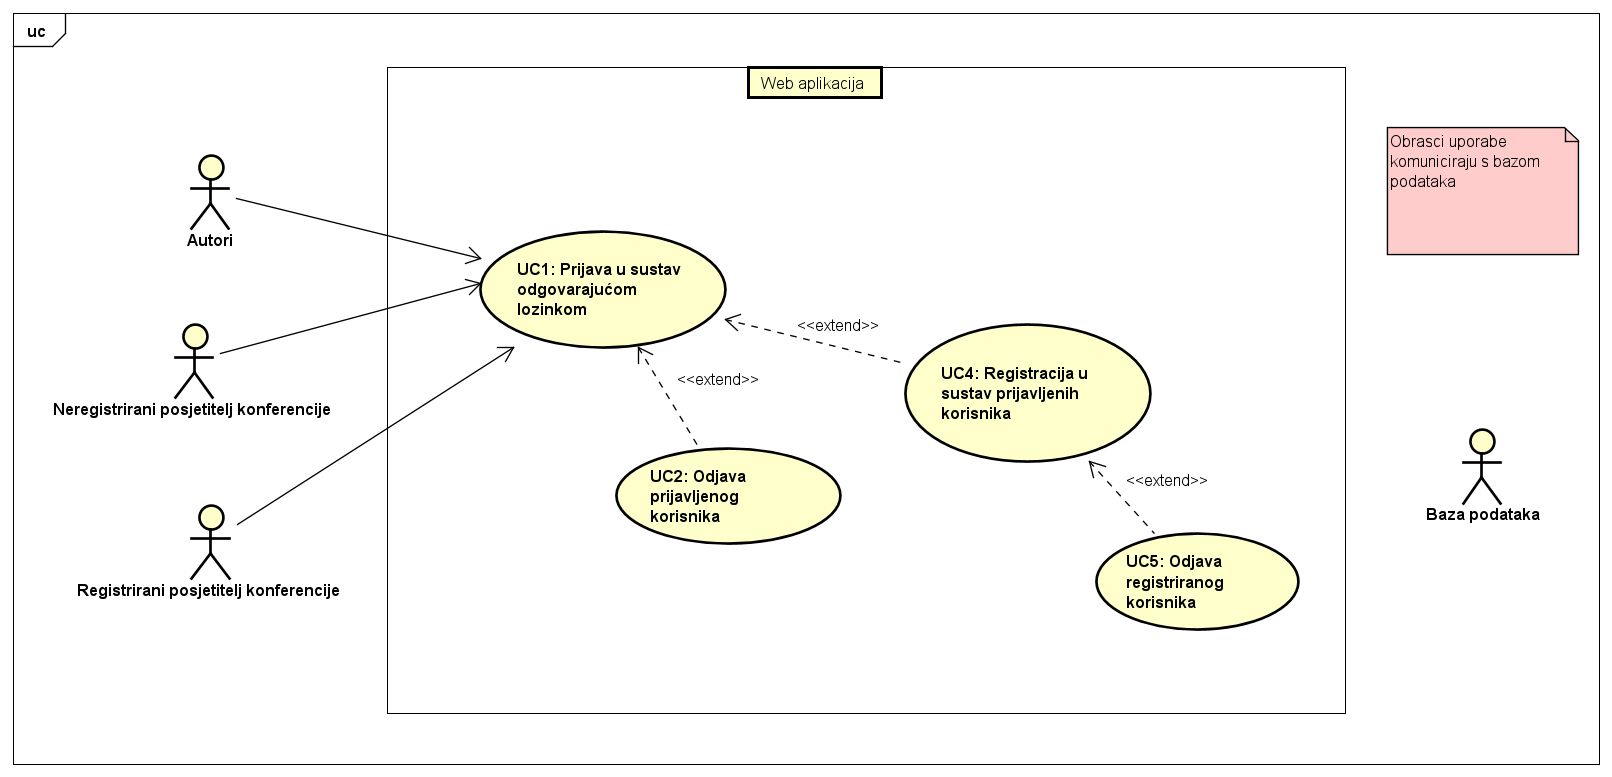
\includegraphics[width=\textwidth]{slike/prijavaUseCase.PNG} %veličina u odnosu na širinu linije
						\caption{Dijagram obrazaca uporabe, prijava u sustav}
						\label{fig:prijava-dijagram} %label mora biti drugaciji za svaku sliku
					\end{figure}
					
					\begin{figure}[H]
						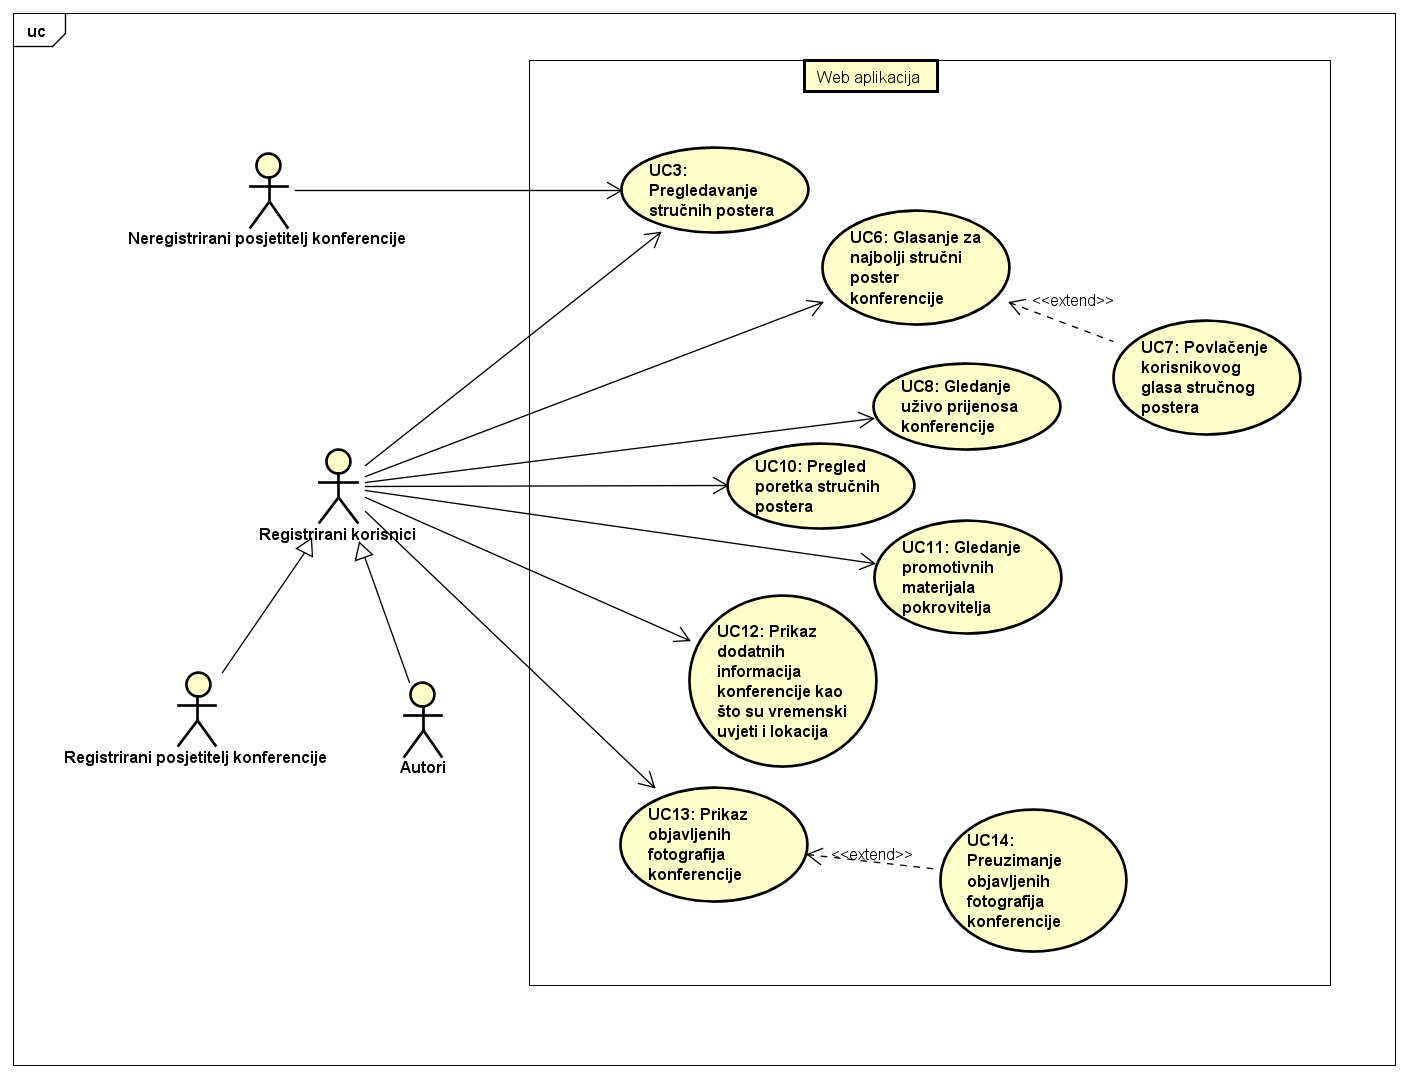
\includegraphics[width=\textwidth]{slike/korisniciUseCase.PNG} %veličina u odnosu na širinu linije
						\caption{Dijagram obrazaca uporabe, funkcionalnosti korisnika}
						\label{fig:korisnik-dijagram} %label mora biti drugaciji za svaku sliku
					\end{figure}
					
					\begin{figure}[H]
						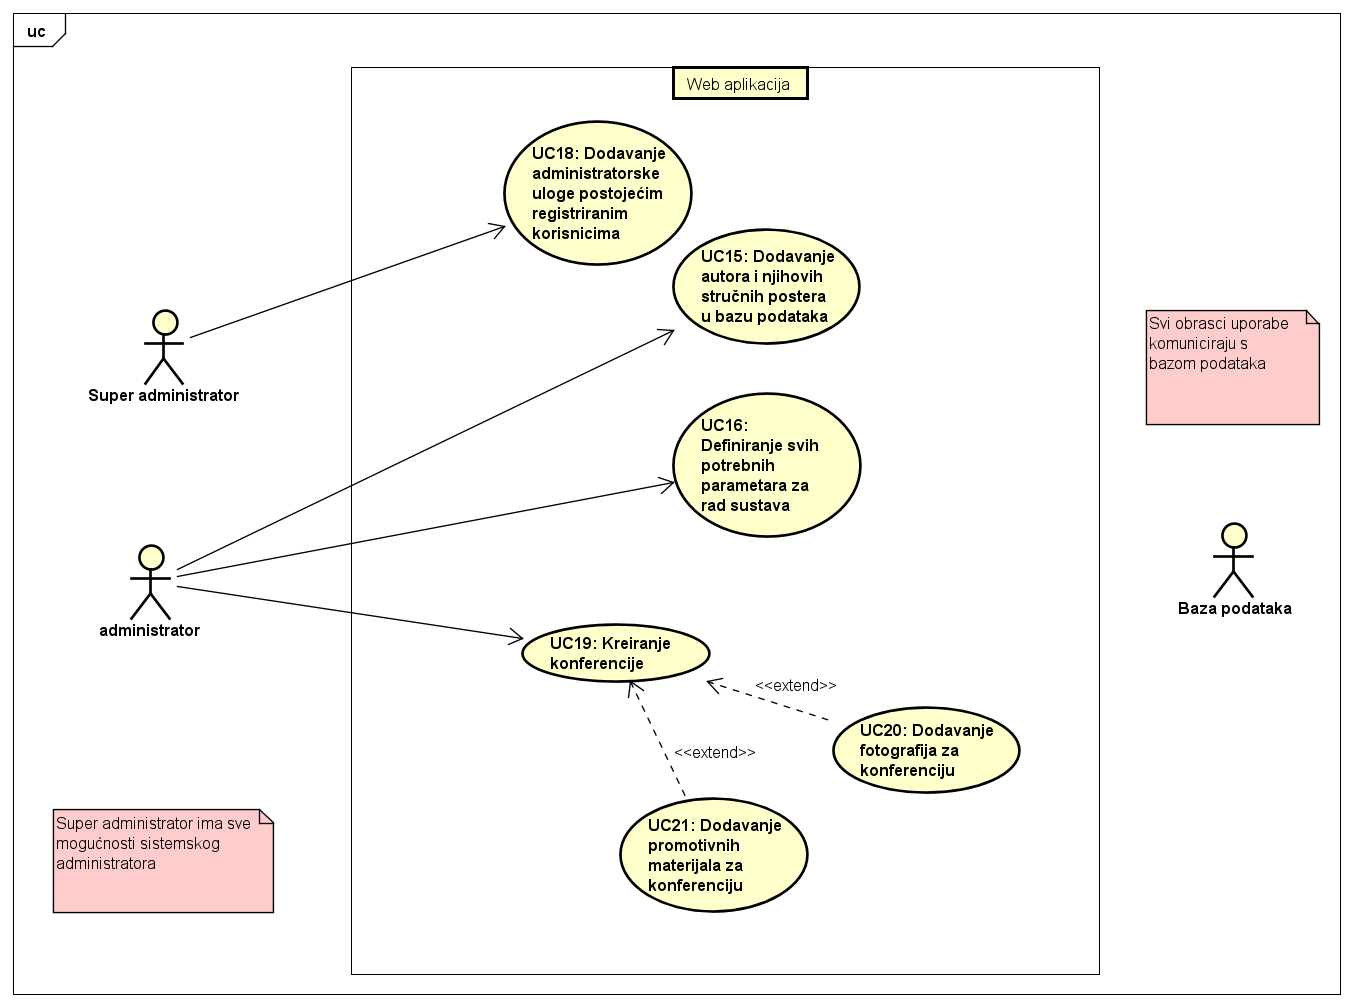
\includegraphics[width=\textwidth]{slike/adminUseCase.PNG} %veličina u odnosu na širinu linije
						\caption{Dijagram obrazaca uporabe, funkcionalnosti administratora}
						\label{fig:admin-dijagram} %label mora biti drugaciji za svaku sliku
					\end{figure}
					
				\eject		
				
			\subsection{Sekvencijski dijagrami}
						
				\textbf{Obrazac uporabe UC1: Prijava u sustav odgovarajućom lozinkom}\\
				Korisnik na početnom zaslonu upisuje lozinku konferencije, te ju šalje poslužitelju. Poslužitelj šalje upit bazi podataka i provjerava je li lozinka ispravna, ako je neispravna ovaj postupak se ponavlja do upisa točne lozinke. Ako je unesena lozinka ispravna korisniku se potvrđuje da je unio ispravnu lozinku, te se od baze podataka zatražuju podaci o konferenciji i oni se šalju korisniku.
				
				\begin{figure}[H]
					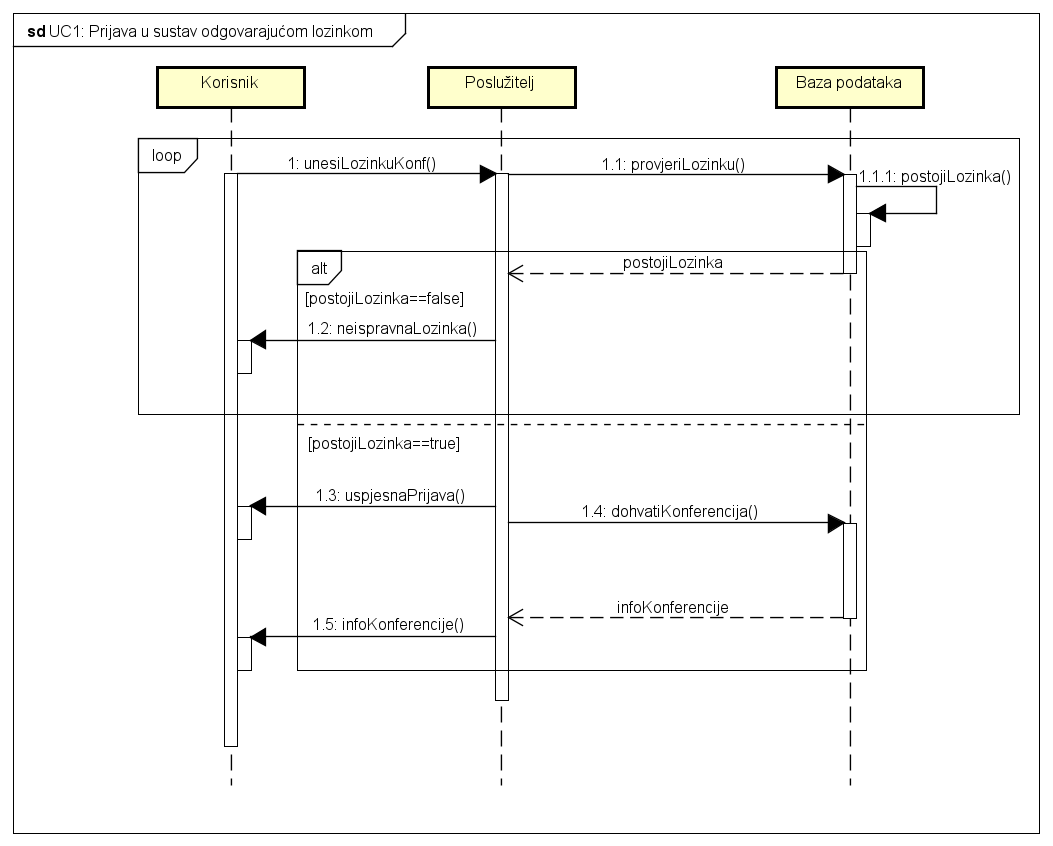
\includegraphics[width=\textwidth]{slike/uc1Sekvencijski.PNG} %veličina u odnosu na širinu linije
					\caption{Sekvencijski dijagram obrasca UC1: Prijava u sustav odgovarajućom lozinkom}
					\label{fig:uc1-sekvencijski} %label mora biti drugaciji za svaku sliku
				\end{figure}
				\eject
					\textbf{Obrazac uporabe UC4: Registracija u sustav prijavljenih korisnika}\\
				Korisnik klikom na gumb registracija pokreće postupak registracije. Sustav mu šalje nazad formu za registraciju u kojoj upisuje email i lozinku i šalje ih sustavu. Zatim sustav provjerava format email-a, ako nije valjan obavještava korisnika o tome, inače nastavlja dalje i provjerava ispunjava li lozinka format, te u slučaju da ne ispunjava također obavještava korisnika. Na kraju se upitom nad bazom provjerava da li postoji registrirani korisnik s tom email adresom. U slučaju da postoji obavijestiti ćemo korisnika o tome, ako ne lozinka će se kriptirati i spremiti zajedno s email-om u bazu podataka i korisnika ćemo obavijestiti da je registracija bila uspješna.
				
				\begin{figure}[H]
					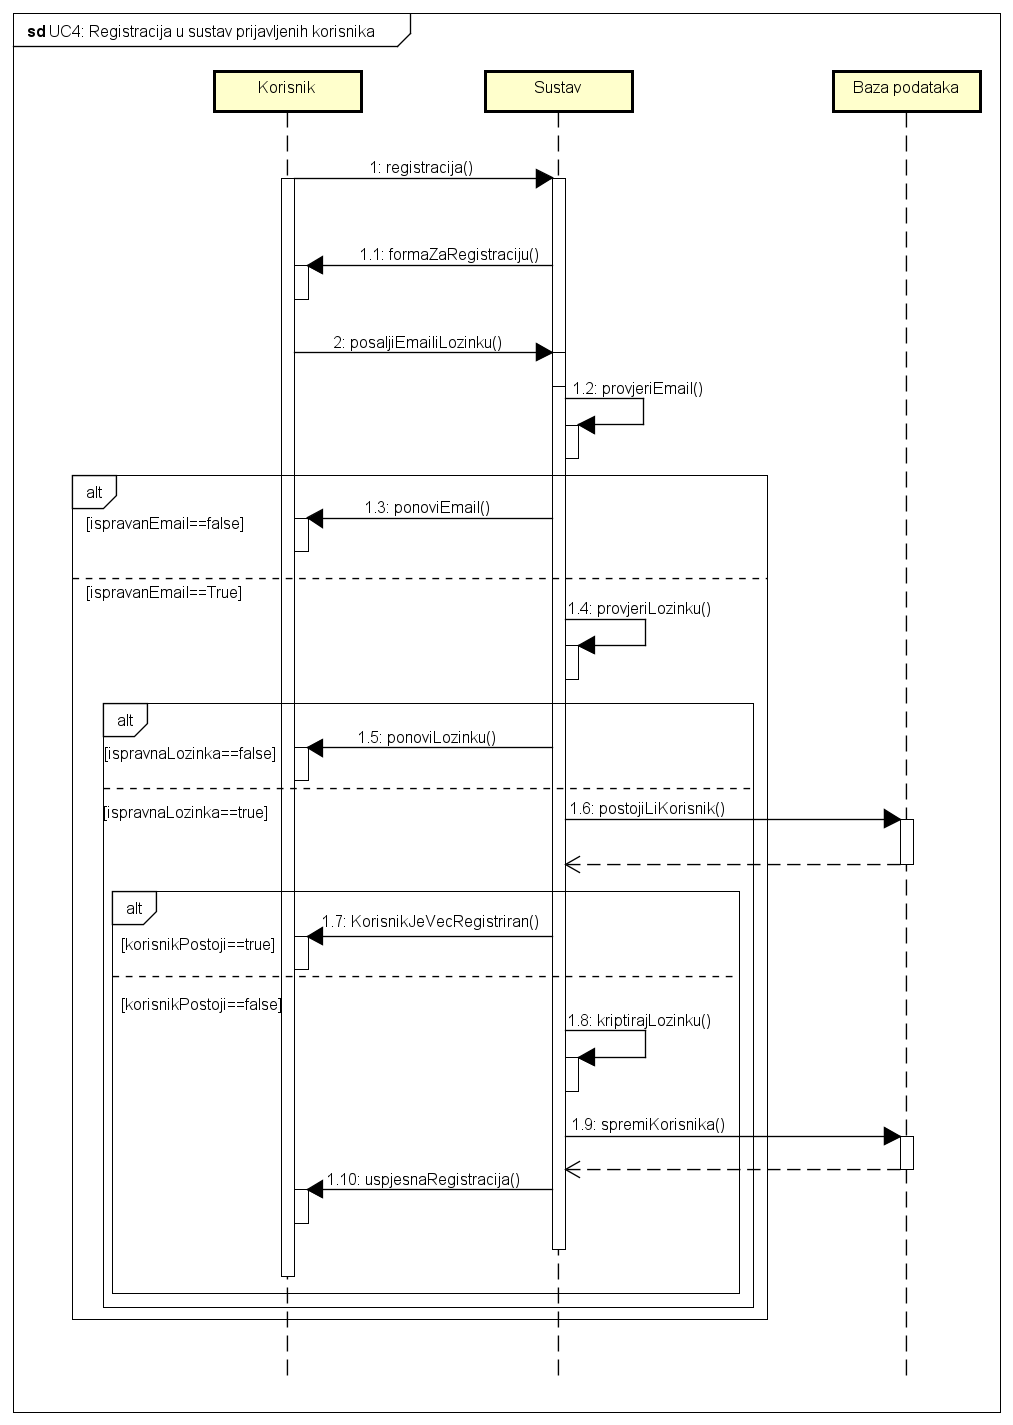
\includegraphics[width=\textwidth]{slike/uc4Sekvencijski.PNG} %veličina u odnosu na širinu linije
					\caption{Sekvencijski dijagram obrasca UC4: Registracija u sustav prijavljenih korisnika}
					\label{fig:uc4-sekvencijski} %label mora biti drugaciji za svaku sliku
				\end{figure}
				\eject
				
		\section{Ostali zahtjevi}
		 
			  \begin{packed_item}
			 	\item Unutar sustava mora biti omogućen istovremeni rad svih korisnika samog sustava
			 	\item Aplikacija se mora moći koristit unutar bilo kojeg web preglednika 
			 	\item Aplikacija se mora ostvariti objektno orijentiranim pristupom programiranja
			 	\item Aplikacija mora biti jednostavna i intuitivna za korištenje svim korisnicima svih uzrasta i predznanja
			 	\item Aplikacija mora biti javno dostupna
			 	\item Unutar aplikacije mora se provoditi autentifikacija te prikazivani sadržaj mora odgovarati dozvoljenom sadržaju za trenutnog korisnika
			 	\item Nadogradnjom postojeće aplikacije ne smije doći do urušavanja funkcionalnosti i kvalitete već postojeće aplikacije
			 	\item Unutar sustava mora biti omogućen unos svih posebnih slova referentnih za odabrani jezik aplikacija (za slučaj hrvatskog jezika, mora biti moguć unos dijakritičkih znakova)
			 \end{packed_item}
			 
			 
			 
	